\section{Why model the brain?}
Diseases of the brain are very widespread and cost world governments a significant amount of money \cite{who}.
The 2015 Global Burden of Disease study estimates that about a third of the population worldwide is affected by mental or neurological disorders across their lifespans
Disorders of the brain rank among the leading causes of ill-health and disability and account for 35\% of Europe’s total disease burden with a yearly cost of 800 billion euros, of which 60\% are related to direct health care and non-medical costs.4,5 % %https://www.who.int/bulletin/volumes/96/5/17-206599/en/ 
\subsection{Computational Models}
In addition to producing actions and goal directed behaviors, the mammal nervous system filters and processes signals in steps that are increasingly understood at mechanical and algorithmic levels \cite{marr1976understanding}.
The recent success of "deep-neural networks" and "recurrent neural networks" is due in part to the simple application of rudimentary neural design principles to networks of computational units.
Innovations in artificial intelligence (AI) have been achieved by recapitulating just a few such algorithms observed in the brain.
For example, artificial neural networks trained to navigate a landscape spontaneously exhibit the emergence of nodes (cell analogues) exhibiting the same behavior as so-called "grid" and "place" cells that encode spatial location in mammalian brains \cite{banino2018vector}.

However, further progress in both human health and artificial intelligence is likely to require a greater understanding of how the brain actually works.
Biophysically realistic computational models of neurons and neural circuits have emerged as useful tools to elucidate brain function in health and disease.
Developing and testing these models may be required to give programmers and engineers insight into the neural principles that underlie human learning and reasoning, so that these principles can be implemented in an electronic substrate.
Because improvements in AI directly contribute to improvements in robotics, and because computers and robots can perform some unsafe and repetitive tasks with high precision, substantial gains in global economic productivity are at stake.
AI may also help to push the frontier of scientific research itself.
%big claims too hard to defend, and to solve or exacerbate existential problems facing humanity.
Our medical understanding of the brain, and digital implementations of brain algorithms would likely improve if existing models for neuron and neural circuits were more tractable, conceptually and computationally.

In this thesis I describe and document tools I developed that improve the speed and accuracy of some classes of neural models.
The speed improvements come from the application of reduced modeling framework, largely relying on existing research, although I also identify and exploit some opportunities for faster model dispatch and simulation.
The accuracy improvements--which constitute most of the novelty here--derive from application of optimization techniques to improve the agreement between models and corresponding "wet lab" experiments in biological neurons.
By improving single cell models, these tools will also serve as a basis for improved neural circuit models, of which many neuron types are among the components.
Since network models many consist of many thousands (or more) of cell models, both speed and accuracy are essential.
\\
% https://www.sciencedirect.com/topics/immunology-and-microbiology/whole-cell-patch-clamp
% Whole Cell Patch Clamp

\subsection{Simulation as Experimental Platform}
The human brain is inaccessible to many experiments for technical and ethical reasons.
Neuroscience relies instead on "model systems" for understanding the human brain.
One such model system is the animal model (or which there are many), chosen due to biological similarities to the organization of the human brain, and the relatively smaller ethical issues associated with experimentation.
However, animal models have limitations which can make them scientifically unfavorable
Animal models often involve years of investment, genetic engineering, complex surgery, complicated behavioral learning paradigms.
Many things can go wrong while developing an assay, potentially ruining a costly experiment, and diminishing years of work.
Furthermore, experiments are still limited by technology; arbitrary control of neural activity is generally not tractable.
Therefore causality and identifiability are still major issues.

For example, in a rodent model of Alzheimer's disease, it is possible to investigate rodent behavior for Alzheimer's symptoms, and to attempt to identify associated changes in physiology, such as changes in cell-specific firing rates or circuit dynamics.
However, the density of placement of recording electrode arrays is very limited, and so the read out of brain activity from electrode arrays is sparse.
Immune reactivity and glial scarring may undermine the fidelity of the underlying system, and make such recordings more difficult.
In \emph{in vitro} recordings, recorded cells are susceptible to "run-down" \cite{colquhoun1994ion}, where the membrane of the recorded neuron membrane its ionic complement changes too much from its \emph{in vivo} conditions. 
Cell run-down creates a small time window for learning about cells in animal experiments, fortunately, cell-run down is obviously not. problem for \emph{in-silico} models.

\emph{In-silico} model systems, e.g. computational modeling, represent an alternative approach.
Rather than simply thinking of computational models as systems of differential equations used to describe and represent the biological processes under investigation, we can think of them as experimental platforms.
Much detail will inevitably lost, and a main assumption is that the important features of the biological processes are reflected in electrical activity, e.g. changes in membrane potential, and that other details abstracted out of the model, for example long-term changes to genes and protein expression, are not essential to understand the problem at hand.
This assumption may be reasonable for investigations of short-time scale phenomenon (e.g. instantaneous responses to stimuli) but not longer-time scale ones (e.g: glial cell re-organisation associated with learning new skills \cite{draganski2008training}).

However, all model systems are imperfect; the \emph{in vitro} brain slice is not an \emph{in vivo} brain, and lacks many putatively important features of a real brain, such as long-range connectivity or even complete dendritic trees.
The limitations expressed in the paragraph above may limit measurement quality.
Ultimately, the question is whether result in the model system will translate to the real one, and how and whether a good simulation platform can outperform an \emph{in vitro} animal model system is an open question.
To achieve this, it is likely that the simulation platform will need to utilize model components as faithful to the real, biological system as possible, and thus it is important that reduced neural models are the most faithful to the cell behavior they represent. 

\section{Why model neurons?}
The idea that neurons are the fundamental computational units of the brain dates to the 19th century [cite something from \url{https://en.wikipedia.org/wiki/Neuron_doctrine}].
A large fraction of computational models have thus included the neuron, at some level of abstraction.  
Conventionally, each neuron has been regarded as an independent generator of events (e.g. synaptic conductances or currents in postsynaptic neurons) and selective receiver of the same events, these inputs summed in some fashion across time and space. 

Although cortical neurons have many interconnections [cite something about cortical connectivity], these connections themselves are plastic, changing with development and learning.
In contrast, the dynamics of the neurons themselves are typically considered less variable over most relevant timescales, i.e. the parameters of the underlying equations may be fixed.
Consequently by placing static neurons at the center of modeling efforts, and letting only synapses change over time, one can still model a large number of relevant neuroscience problems.
But just because the modeled neurons are static does not mean they are monolithic: there are many thousands of different classes of neurons, each with its own idiosyncratic dynamics and connectivity.
And many such classes might be essential for the generation of even simple behaviors.
Therefore understanding the brain may require the ability to accurately model not just neurons per se, but many kinds of neurons.

Alternatively, one could model subcellular processes to get an even more accurate picture of biology than is obtained from considered the neuron as the basic unit of the brain.
However, this greatly increase computationally complexity, is even more limited by the availability of experimental data (or theory) on the relevant processes, and is an open question whether such detail improves the predictive or explanatory accuracy of models anyway.
Simplifying assumptions are often needed in modeling, and the simplifying assumption that I choose here is to abstract away these subcellular processes into a small number of state equations that describe observable physiology at the whole cell level.

One could also model above the level of neurons, by creating mean-field and population models of brain tissue.
However, this makes it difficult to understand intra-circuit computations occurring in local circuits, or to understand how a change to e.g. a single conductance might affect a behavior.
Some also argue that spiking is necessary per se to reproduce some kinds of population dynamics, especially those that evade intuitive understanding.
And model-as-simulation-platform is less compiling if the outcomes of the simulations are obvious in advance.

% - How are neurons modeled (i.e. math and equations)
\subsection{Conductance Based Models}
Conductance-based models are mathematical representations of the electrical and chemical behavior of semi-permeable neuronal membranes.
The phospho-lipid membrane of neurons, otherwise a insulative capacitor, contains a variety of conductive pores (ion channels), each permitting the passage of specific ions at specific rates.
These rates are determined by free energy gradients, jointly determined by transmembrane ionic concentration gradients (entropy) and on the transmembrane voltage voltage changes adjacent to the channel (potential energy).
In conductance-based models ion channels are represented as differential equations that explicitly represent the rate at which specific ionic species flow through each channel type at each location on the neuron, i.e. ionic currents.
Conductance-based models differ in their spatial extent. In its most basic form, a conductance based model can describe an isoelectric sphere (in this case the model is so abstract that it dispenses with the notion of space in nervous tissue).
In a large variety of conductance based models, the 3D form of neural membrane is "modelled", but it is approximated by using elaborate systems of 2D branching patterns \cite{rall1962electrophysiology}.
Rall pioneered application of numerical methods of the $3D$ Hodgkin-Huxley models, Rall took numerical methods used for modelling heat and electrical conductance in cables, electrical distribution of charge in a cable and showed that similar equations could be used to accurately predict current flow in the cable of neuron dendrite.
\\
\begin{center}
\begin{equation}
I_{m(t)}=I_{C}+I_{ionic} 
I_{C}=C_{m}\frac{dV(t)}{dt} 
I_{ionic}=I_{Na}+I_{K}+I_{L}
\end{equation}
\end{center}
\begin{equation}
I_{ionic}=\\
g_{Na}(V)[V(t)-V_{Na}]+\\
g_{K}(V)[V(t)-V_{K}]+\\g_{L}[V(t)-V_{L}] 
\end{equation}
In the context of realistic 3D modelling, conductance based models are very slow to solve because they contain many (tens or more) coupled differential equations which must be solved at every discrete location across the neuron.
These locations (segments) may have unique parameters, as simple as segment diameter (corresponding to e.g. tapering of dendrites) or as complex as distance-dependent changes in the distribution of specific ionic conductances.
Many of these fine structural variations are incorporated into biophysically-detailed brain models.  
Because the structure of the "cable" itself changes the neural firing dynamics, even a generic set of principles may result in distinct dynamics across different realizations of the same class of neuron.  
Clearly, there is a large cost in simulation performance and in generalizability.

\subsection{Reduced Models}
Conductance-based models can be complex--both conceptually, in implementation details, and in computational demands--so it is common to employ a variety of simplifications that retain the general input/output behavior of the full model.
These "Reduced Models" ignore the precise neuron biophysics, usually retaining only the medium-time-scale (milliseconds to tens of milliseconds) dynamics by assuming that anything faster occurs instantaneously and anything slower can be ignored.
The 3D structure of biological cells is flattened to a point onto which currents impinge and voltages evolve over time. There is a great diversity of real biological neurons, all of which differ substantially in their electrical behavior. There are a few different classes of general purpose neuronal models, that can reproduce these different types of electrical behaviours, given appropriate parameterizations of the models. A selection of key reduced models is described below.
\subsubsection{The Leaky Integrate and Fire Model}
....
\subsubsection{The Quadratic LIF Model}
...
\subsubsection{The Generalized LIF Model}
...
\subsection{Adaptive Exponential Integrate and Fire Model}
\begin{center}
$C\frac{d}{Vdt}=-g_{L}(V-E_{L})+
g_{L} \Delta Texp(V-V_{T} \Delta T)-w+I$

$\tau_{w}\frac{dw}{dt} = a(V-E_{L})-w $
\end{center}
The Adaptive Exponential (AdExp) IF model \cite{brette2005adaptive}, is another type of reduced neural model
The Adexp model is a special instance of leaky integrate and Fire model which most often appears with an exponential spike shape.
The models instantaneous spiking rate is calculated via a consulting finite time "windows" into the neurons recent spike history.
Adaptation is achieved by looking back into the window and counting the number of spikes that occurred in the previous $10ms$, for example. 
\subsubsection{Izhikevich Model}
An existing class of neuron model type, called The Izhikevich model \cite{izhikevich2003simple} (Iz model) was published with parameter sets believed to make the model outputs accurately align with a variety of real biological cell outputs. However since publication much very specific electrophysiological recordings have accumulated, that in someways undermine model/experiment agreement. However it is now possible to constrain the Izhikevich model and find new parameterizations that more allow us to more accurately reproduce more recently published experimental data.
The original formulation involves the integration of a quadratic function:
$\frac{dv}{dt}=0.04v^{2}+5v+140-u+I$
$\frac{du}{dt} = a(bv-u)$
$if v>=30mV,
then v arrow c u arrow u+ d$
However, an alternative implementation is more versatile, as it can be fitted to a wider range of parameters:
The Izhikevich model and the AdEx model are both related to simple Integrate and Fire model.
The Izhikevich model takes a current injection value, and a capacitive current, a membrane potential is created by integrating an equation $\frac{d V_{M}}{dt}$.
The Izhikevich model has quadratic multiplicative terms.
The GLIF and the AdExp models have exponential multiplicative terms.

Network simulation is only as fast as the slowest model, because (if you are waiting for one neuron to evaluate, the whole network will need to wait, as its state may depend on that neuron).
Consequently, replacing biophyshically detailed models with the reduced models described above may be required to complete simulations in a reasonable amount of time.
However, the accuracy of these models is also paramount.
Yet there are no reports of large numbers of reduced models with demonstrated agreement with many pieces of experimental data.

\subsection{Simulation of reduced models}
Although this model is potentially fast, often python implementations of it are slow due to code that was written to make running populations of many neurons fast, at the expense of running single neurons. 
For instance, Brian2, and a related tool neurodynamics, have code for running AdExp neurons, however brian2 has network c-level Cython code that interferes with DEAP python code.
\\
%Its as if a reduced model is a black box representation of a neuron, and the reduced model is a transfer function that maps inputs to outputs. Typically reduced models are very fast to solve.\\
%\\
% - Kinds of reduced models and what they can do
%\section{Introduction}
% above.
% 2-5pages
\section{Parameter Fitting and Model Optimization}
Model parameters dictate model behavior, but many parameters either (a) cannot be easily measured in experiments for technical reasons or (b) don't even correspond to a theoretically measurable quantity.
As an example of the latter, consider any "emergent behavior" whose observables do not map directly onto any specific model parameter.
In the transition between conductance-based models to reduced models, the number of unknown parameters of form (b) increase relative to form (a).
In any case, these unknown parameter values make specification of realistic model specification difficult.

Simulation corresponds to integrating a model's differential equations to obtain the time-varying values of model state variables.
Some of these state variables may be observable.
In all of the reduced models described above, the only observed state variable is the membrane potential, $V$.
Additionally, there is another state variable $I$, corresponding to somatic current injection, that is under control of the operator of the simulation experiment, and which is (for a single neuron model), independent of all other parameter values or state variables.
If the model is simulated enough times with enough different values of $I$, it may be possible in principle to identify the values of all other parameters by observing the corresponding time-dependent trajectories of $V$.
By analogy, it is possible to solve a system of linear equations when the number of equations is greater than the number of unknowns.

Consequently, one strategy for inferring model parameters, sometimes called "parameter-fitting", is to identify those parameter values which produce state-variable time series which agree (according to some criteria) with corresponding observable experimental measurements.
For example, a common approach for approximating unknown ion channel densities is to ‘optimize’ or iteratively simulated the model, altering the parameters systematically until the simulated time series of $V$ matches some membrane potential trace recorded under similar conditions in an biological neuron.

What does it mean for the simulated and biological time series of $V$ to match?
Recall that both models and biological neurons can be injected with specific amounts of current. Because neurons are electrically excitable, somatic membrane potential departs from resting membrane potential in response to current injections.
For many classes of cells, abundant experimental data exists concerning the responses (membrane potential time series) to each magnitude or shape of somatic current injection.
A crude measure of error would be to simply directly compare the model and biological time series, using the mean-squared-difference, for example.
However, because excitability reflects a non-linear transformation between input and output, this means that very small differences in input (or parameters) can have massive differences on output, especially its timing.
A single action potential shifted by a millisecond (approximately the width of one action potential) might be insignificant from a practical perspective, but produce a massive "error" signal using mean-squared difference.
Consequently, I use an approach based on more robust statistical summaries of the membrane potential, including those believed to be meaningful in neural coding.
These are described in more detail below.

The process of optimization involves what is known as an ‘inverse’ problem.
A naive approach to solving this inverse optimization problem works on the principle of elimination.
A large number of unsatisfactory parameter sets must be sampled, to rule out the possibility that each candidate parameter set is not worse than some currently favored parameter set.
Doing this exhaustively, using a grid search across all combinations of parameter values with sufficient resolution, is often  computationally intractable.
Consider the Izhikevich model above.
In its most general form, it contains 10 tunable parameters.
Evaluating even 25 values of each parameter implies $25^10$ parameter sets, or nearly 100 trillion parameters sets.
Even if 1 million could be checked every second, this would still take 3 years.
And the cost grows exponentially with increases in parameter resolution or number.

Fortunately, shortcuts exist whose utility depends on the shape of the so-called "error surface".
For any specific instance of a model, with a given set of parameter values, its suitability is evaluated according to some "objective function" that compares the simulated output under one or more conditions to some corresponding experimental data.
By convention, the objective function may report this suitability as an error metric, minimal when the simulated and biological results disagree to the smallest extent possible (which may not be zero, see below).
Model "optimization" then corresponds to finding the parameter set which minimizes this objective function. 
Because the objective function returns a measure of error, the "error surface" corresponds to the output of the objective function for each possible set of parameter values.
Ideally, this surface is perfectly "convex", meaning that there is a single minimum, and from any starting point one can follow some variant of a gradient descent strategy to find that minimum.  

\subsection{Local Minima} Many real optimization problems have error surfaces that not perfectly convex but are instead actually have a surface shape that is rippled, so that as you travel along the error surface in any direction, you may encounter multiple troughs of similarly low error value (local minima).
These ripples make navigating the error surface non trivial.
Rastrigin's function [insert figure reference] is a function for creating error surfaces to test the robustness of algorithms that attempt to overcome this problem.
The surface described by the function is densely populated by local minima, each of which is placed on a globally convex envelope, such that the true minimum of Rastrigin's function is at its centre.

\subsection{Genetic Algorithms}
A variety of numerical optimization techniques exist, and which performs best depend on the demands of the problem.
For functions with many local minima, it is often best to broadly sample the error surface, rather than attempt a "greedy" search for the global minimum.
Several notable algorithms including genetic algorithms and stochastic gradient descent (SGD) have been developed to address this use case.
Both of these algorithms are able to avoid putting all of their "eggs" in one local minimum "basket", allowing them to discover over many iterations that are a lower minimum is available.
For example, given enough samples a genetic algorithm will learn the global minimum of the Rastrigin's function, although it is very likely to sample wells spanning many depths of the error function on the way down.

% illustrate how a Genetic Algorithm (GA) generally works.
\begin{center}
\begin{figure}
    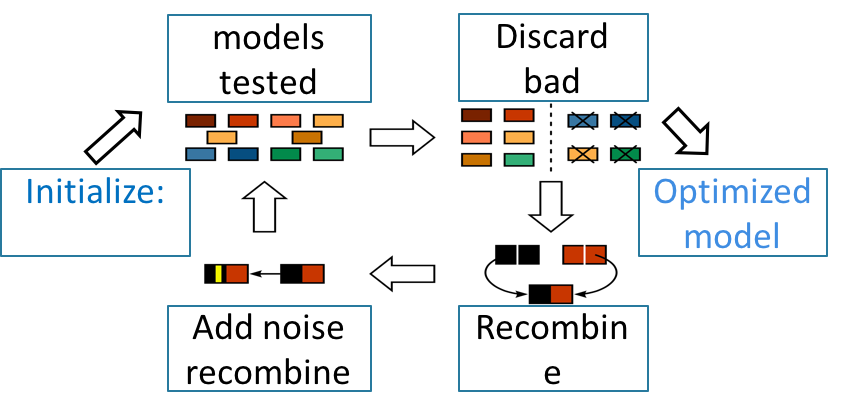
\includegraphics[width=0.7\linewidth]{figures/How_Genetic_Alg_Works.png}
  \caption{Genetic algorithms find satisfactory solutions by incompletely sampling the solution space. Evolution of the algorithm is guided by the combined application of stochastic sampling and selective pressure. Stochastic contributions that guide GA sampling incentivise the exploration of regions beyond local minima. Stochasticity is applied in the combined actions of cross-over, and mutation. Model parameterizations are encoded as binary strings called genes. When genes breed, eligible pairs of genes are aligned and at random bit locations, the status of a bit is exchanged.  
}
  \label{fig:GeneticAlgOver}
\end{figure}
  
\end{center}

I use genetic algorithms in the work presented here, and while there are many variations on this approach, they all involve some combination of the following features:
% My GA picture belongs here
\subsubsection{Chromosomes}
In the context of genetic algorithms, a chromosome is the complete set of model parameters that are necessary to fully define the model being optimized, in this case a neural model.
These parameter sets are collections of floating point numbers, for example -65.7 for a reversal potential in mV.
\subsubsection{Genes}
In the context of genetic algorithms, a gene is a single model parameter.  Consequently, the number of genes in a chromosome is equal to the number of parameters in the model.
There are at least two stochastic operations that over time provide a gentle "exploratory drive" for the algorithm, that cause genes to either double down on exploration of a local minimum, or possibly "jump" out of a local minimum to realize lower error.  These operations are applied, with some user-determined frequency, with each "generation" of the population of chromosomes, to determined the members of the subsequent generation.
\subsubsection{Simulated Genetic Recombination: Cross-over}
Cross-over is the exchange of genes between chromosomes.  In a population of many chromosomes, one can "mate" two of them, producing off-spring which represent a fraction of genes from parent 1 and the remainder from parent 2.  If each chromosome represents two opposing vertices of an n-dimensional hypercube (for n model parameters), then cross-over is capable of producing offspring representing any of the other vertices in that hypercube.
\subsubsection{Simulated Genetic Mutation}
A mutation reflects a (random) change to a single gene, i.e. a change to a single model parameter.  In some implementation this is achieved by flipping one bit in the binary representation of the floating-point value of the parameter, with the magnitude of the resulting change in the parameter value depending on which binary digit was flipped.  Often mutation is limited to a particular range for a given parameter.
\begin{center}
\begin{figure}
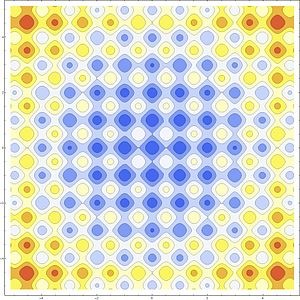
\includegraphics[]{figures/rastagrind}
\caption{Rastrigin's function is a function that is challenging to optimize, as it contains thousands of local optima which would trap a gradient descent algorithm}
\end{figure}
\end{center}

\subsubsection{Elitism}
The number of chromosomes in each generation is typically fixed, with some chromosomes in generation n+1 coming from crossover of chromosomes in generation n and others from mutation.
The remainder are often chosen from the fittest, i.e. lowest error, members of generation n, a strategy known as elitism.
The degree of elitism essentially controls the amount of evolution that is allowed to occur in each generation.

\subsection{Multi-objective optimization} Multi objective optimization problems are a subset of optimization problems.
In a multi-objective optimisation model fitness is evaluated using multiple "objective functions" of model fitness, each contributing either independently or in conjunction to the error surface.
Each function may ask a different question about the model; for example, one may ask how well the model reproduces the shapes of action potentials, and another function may ask how well the model reproduces the counts of action potentials.
The output of each such function is some scalar, with a lower value representing greater model/data agreement, i.e. lower error.
These functions are sometimes also called constraints.

\subsubsection{Weighted optimization} simple strategy is to turn a multi-objective optimization problem into a single objective optimization problem, for example by summing the outputs of objective functions together. 
This is an extremely common strategy, has been the dominant approach in all neuroscience model optimization efforts to date [cite something here].
However, this comes with a significant price.
Optimization using a sum over multiple error measurements leads to a situation where a single constraint has an especially deep error surface, such that the gradient of the overall summed error surface is dominated by that single constraint.
In other words, minimizing overall error mostly corresponds satisfying only one constraint.
The optimizer invests most of its search effort achieving a low error on one constraint, leaving the others unacceptably high.
This problem can in principle be ameliorated by re-scaling the objective functions to have similarly deep error surfaces, but in general the shapes of the error surfaces cannot be known in advance, so this sort of approach cannot generalize.\\

\subsubsection{Non-dominated Sort} A less appreciated but perhaps more important drawback to collapsing multiple objectives to a single one is that it imposes an opinion about the relative importance of each objective.
However, while there may underlying "true values" for measured biological variables, there is no underlying truth about which variables are more important than others.
In problems where not all measurements can be perfectly replicated by models (in part because the models are inherently simplifications of biology), this problem becomes even more pressing.
The experimental data themselves may also come from multiple data sources, so the solutions corresponding to each single objective actually reflect the diversity of the underlying system (e.g. physiological diversity of neurons of a given type), which is lost when this is collapsed to a single objective.

A multi-objective optimization paradigm that admitted diverse sets of solutions to a list of constraints might better reflect real biology while also imposing less opinion about which measurements are most important.
The so-called "Non-dominated sort" is one such paradigm.
It considers each objective function separately, and only considers one chromosome to be superior to another if it "dominates" that other, meaning that the objective function output is lower (i.e. smaller error) for each objective function.
If even a single objective function has a larger value for the latter chromosome, then it is not dominated.  Any chromosome that is not dominated by any other chromosome is considered "non-dominated" and is retained (i.e. for mutation, cross-over, or elitist selection) into the next generation.

The non-dominated set of chromosomes has a simple interpretation: each of its members would minimize a single, weighted objective function for some set of weights.
If no other chromosome has strictly equal-or-lower objective function evaluation for all constraints, then there exists a linear combination of weights which would give that chromosome the minimal evaluation (minimal error, maximal fitness) across the entire population.
Thus, retaining this population is equivalent to retaining all possible "opinions" about appropriate weights for the entire optimization process.

The NSGA2 algorithm [insert citation] is a common implementation of this strategy, and is used throughout this work.  Its performance can be compared to, for example, an exhaustive "grid search" across sets of model parameters, at least in low dimensions.  

\subsection{The Curse of Dimensionality}
Brute-force exploration of parameter space requires computation time that scales exponentially with the number of parameters.  In contrast, more efficient searches can be polynomial (e.g. linear or quadratic) in dimension number.  However, if constraints are weak, or conflicting, or the error surface is especially non-convex, many of these gains are lost, and exponential search times may return.  Thus, there is no guarantee in advance that reduced model optimization, with existing experimental data, is a problem that can be reasonably solved for sufficiently high-dimensional reduced models.

% First include a section about NeuronUnit more generally.  NeuronUnit really isn't/wasn't about optimization until your thesis.  
\section{Data Fitting and Optimization with NeuronUnit}
My lab previously developed a Python package called "SciUnit" for scoring scientific models according to their agreement with various experimentally-derived data (encoded as "validation tests") [cite Omar et al 2014].  These scoring process is the implementation of the objective function that I use here.
In particular, I used a SciUnit-based python library called "NeuronUnit" which provided a number of such validation tests for neuron models, and developed additional such tests in the course of my research.

\subsection{Constraint scoring}
The scoring mechanism within these tests determines the output of each objective function to be minimized.  There are many candidate scoring mechanisms, depending on what one means by "the model agrees with the data".  Each first computes some summary of model output, for example the resting membrane potential, called a "feature".
I used two scoring mechanisms most frequently: (1) compute the ratio between the model output feature and the experimental data feature mean, and (2) compute a Z-score reflecting the normalized distance between the model output feature and the distribution of experimental data features.
In both cases, the relevant experimental data distribution might be within trials, across trials, across cells, or even across labs, producing many sources of hetereogeneity.
For example, resting membrane potential (measured in $(mV)$), may vary in some dataset according to a distribution with a mean and standard deviation of $(\mu,\sigma)=(-65mV,15mV)$.
The optimizer may sample a model (with some parameters) with a simulated resting potential of $-68mV$.  
NeuronUnit would then use these values to compute a Z-Score of $(-68 - (-65)/15 = 0.2$.
A model with a Z-Score of 0 would reflect perfect agreement with experimental data, and very low or very high values would represent poor agreement.
Our lab previously showed models can be scored on very large numbers of such tests, corresponding to experimental data for particular neuron types, and used to build biophysically detailed neuron models for the mammalian olfactory bulb [cite Birgiolas thesis].

\subsection{Data aggregation}
NeuronUnit thus converts a quantitative measure of model/data agreement into a useful error signal that can guide model optimization.
But a second function of NeuronUnit is to aggregate the relevant experimental data itself, in order to make  construction of the tests described above possibles.
And a third function is to apply some signal processing and feature extraction steps to these data in order to produce something that can be scored.
This features were present at the beginning of this project, but I have extended them to cover more datasets and more features, as described in the Methods.

\section{Model Simulation and Exchange}
The NEURON simulator is a software suite that wraps powerful and fast ordinary differential equation solvers based in the C programming language inside a mixed compiled/interpreted environment targeted at research scientists. NEURON is somewhat analogous to older, analog circuit simulators;
however, rather than describing complex resistor-capacitor circuits, NEURON instead solves equations for the time varying membrane potential of multi-compartment models.

In contrast to reduced models, multi-compartmental models digitally encode the form of membrane tissue: cables of varying diameters and lengths that represent the morphology of neurons, and these cables support smaller scale representations of ion channels, and ion currents in the membranes.
These neuronal models can be coupled together into a network, where the electrical state of one neuron has an impact on the state of coupled neurons through synaptic currents.
Specifying the system of differential equations representing these neuronal morphologies, ion channels, and synaptic connections is complicated, but NEURON makes multi-compartment neuron simulation efficient, convenient, and achievable.
Models expressed in NEURON code are procedural in nature, and the code consists of low-level implementation details.
Procedural descriptions of models are difficult to extend and re-use, leading to a need for a declarative model description language.

NeuroML is an extensible markup language (XML) tasked with describing these complex network models.
In principle, any simulation (not just NEURON) can execute a simulation based on a NeuroML file, so NeuroML models are readily executed across different types of simulators (ideally with identical results).
This facility makes NeuroML an excellent format for model sharing, and permits cross-examination of results if they vary across simulators, but also allowing different modeling communities to retain the tools that they know best.
Because NeuroML is extensible and component based, it also incentivizes a "plug-in" environment for including pre-existing model components in models in different large-scale contexts.
These components can include complete reduced models, for examples embedded into larger neural circuits.

However, NEURON focuses on efficient simulation of multicompartmental models, and NeuroML on model exchange. 
Neither tool was designed with the optimization of reduced models in mind.
In optimization, the same model may be re-executed hundreds of thousands of times (with different parameter sets), so any computational overhead (for example, associated with reading/writing a file) is quite costly.  
There are other tools that may result in faster optimizations, but as I show here, even these are not optimally fast.
Consequently, it is best to think of tools like NEURON and NeuroML has useful for optimized models, but not necessarily for the optimization itself.  

\section{Analysis of Model and Experimental Variance}
It is common to observe large variations in measurements of a single electrophysiological entity from neurons of the same classification \cite{tripathy2014neuroelectro}.
For example, measured input resistance may be different when recorded from different instances of cerebellar Purkinje cell.
Such differences may be due to differences in experimental methods across organisms, investigators, or simply due to finite random sampling.  
Aggregated data may have been collected from mice, rats, marmosets, macaques, or even humans.
Human data may have been collected under any number of disease states.

Understanding and modeling within-type variation should be considered an essential component of the scientific merit of computational modeling of a neuron-type.
However, the impact of this experimental variation on the production of cell-type-specific models has not previously been explored.
Consequently, I will present here a large-scale analysis of the consequences of this variability--across many electrophysiological features--on the effort to produce canonical reduced models of several common neuron types.
We would like to understand whether the space of existing or potential neuron models accurately represents the variability in the actual experimental data, and to help researchers map data collected from a number of experimental preparations onto a standardized rodent electrophysiological phenotype space.

\subsection{Relationship between Missing Data Imputation and Optimization}
Existing data sets are incomplete, consisting of a sparse sampling of cells in the rodent brain. By necessity, models are constrained using these incomplete data sets.
These missing data occur at multiple levels including exact neuron to neuron wiring patterns, un-sampled morphologies, unknown synapse activation times, and unknown axon and dendrite synapse locations.
More relevant to reduced models, even very basic information about spiking patterns in response to simple current injections may be unavailable.
However, since most fast numerical methods are incompatible with missing data, an additional component of model development--especially in the context of optimization--remains, which is the synthesis of plausible missing values.

\subsection{Closed Loop Development}
The speed of simulation is a critical to successful optimization. However, even when using High Performance Computing (HPC) resources, errors may arise, and require special handling or visualizations to diagnose.  
These errors may even reveal that the model is mis-specified, but this may not be revealed until thousands of simulations have already run.
The ability to address and correct such mistakes, requires rapid and verbose feedback during optimization, as well as simulations of sufficient speed that since error "breakpoints" can be reached in a reasonable amount of time.

\subsection{Successful Optimization} 
Integrating the above ideas, I aimed to develop a framework for rapid, debuggable optimization of reduced neuron models subject to multiple constraints forged by real experimental data, and to use this framework to optimize and share such models.
Here I will describe a number of methods and simulation experiments which demonstrate the successful implementation of many of these ideas, focusing on genetic algorithms that retain a diverse set of model parameterizations, potentially reflecting real within-type neuronal diversity.
The interaction between model constraints cannot always be known in advance, and in fact some constraints are mutually exclusive, causing optimization to fail.
I also aimed to catalog such cases and use this knowledge to produce a more robust set of constraints, implemented via NeuronUnit tests, for future optimization work.

No model--including those that are published-- should not be regarded as final.
Instead, I aimed to develop tools to improve these models by making them agree with experimental data, in the hopes that such models may be of general use to the neuroscience community in future work.
